%%%%%%%%%%%%%%%%%%%%%%%%%%%%%%%%%%%%%%%%%%%%%%%%%%%%%%%%%%%%%%%%%%%%%%%%%%%%
%%%%%                          ANNEXE 1                               %%%%%%
%%%%%%%%%%%%%%%%%%%%%%%%%%%%%%%%%%%%%%%%%%%%%%%%%%%%%%%%%%%%%%%%%%%%%%%%%%%%

\appendix
\renewcommand\chaptername{Appendix~}
\phantomsection 

\lhead[\fancyplain{}{\leftmark}]%Pour les pages paires \bfseries
      {\fancyplain{}{}} %Pour les pages impaires
\chead[\fancyplain{}{}]%
      {\fancyplain{}{}}
\rhead[\fancyplain{}{}]%Pour les pages paires 
      {\fancyplain{}{\rightmark}}%Pour les pages impaires \bfseries
\lfoot[\fancyplain{}{}]%
      {\fancyplain{}{}}
\cfoot[\fancyplain{}{\thepage}]%\bfseries
      {\fancyplain{}{\thepage}} %\bfseries
\rfoot[\fancyplain{}{}]%
     {\fancyplain{}{\scriptsize}}


%%%%%%%%%%%%%%%%%%%%%%%%%%%%%%%%%%%%%%%%%%%%%%%%%%%%%%%%%%%%%%%%%%%%%%%%%%
%%%%%                      Start part here                          %%%%%%
%%%%%%%%%%%%%%%%%%%%%%%%%%%%%%%%%%%%%%%%%%%%%%%%%%%%%%%%%%%%%%%%%%%%%%%%%%

\chapter{Appendix A : Title}
\label{Ann:1}

%==============================================================================	Résumé du chapitre

\begin{center}
\rule{0.7\linewidth}{.5pt}
\begin{minipage}{0.7\linewidth}
\smallskip

\textit{
Supplementary figures for Chapter 4 on \nameref{ch:4}, for the running and cycling tasks. \newline\newline All details on methods and results are provided in the forementioned chapter.
}

%\smallskip
\end{minipage}
\smallskip
\rule{0.7\linewidth}{.5pt}
\end{center}

%\adjustmtc
\minitoc
\newpage


\begin{figure}[!ht]
	\centering
	\def\svgwidth{1\columnwidth}
	\fontsize{10pt}{10pt}\selectfont
	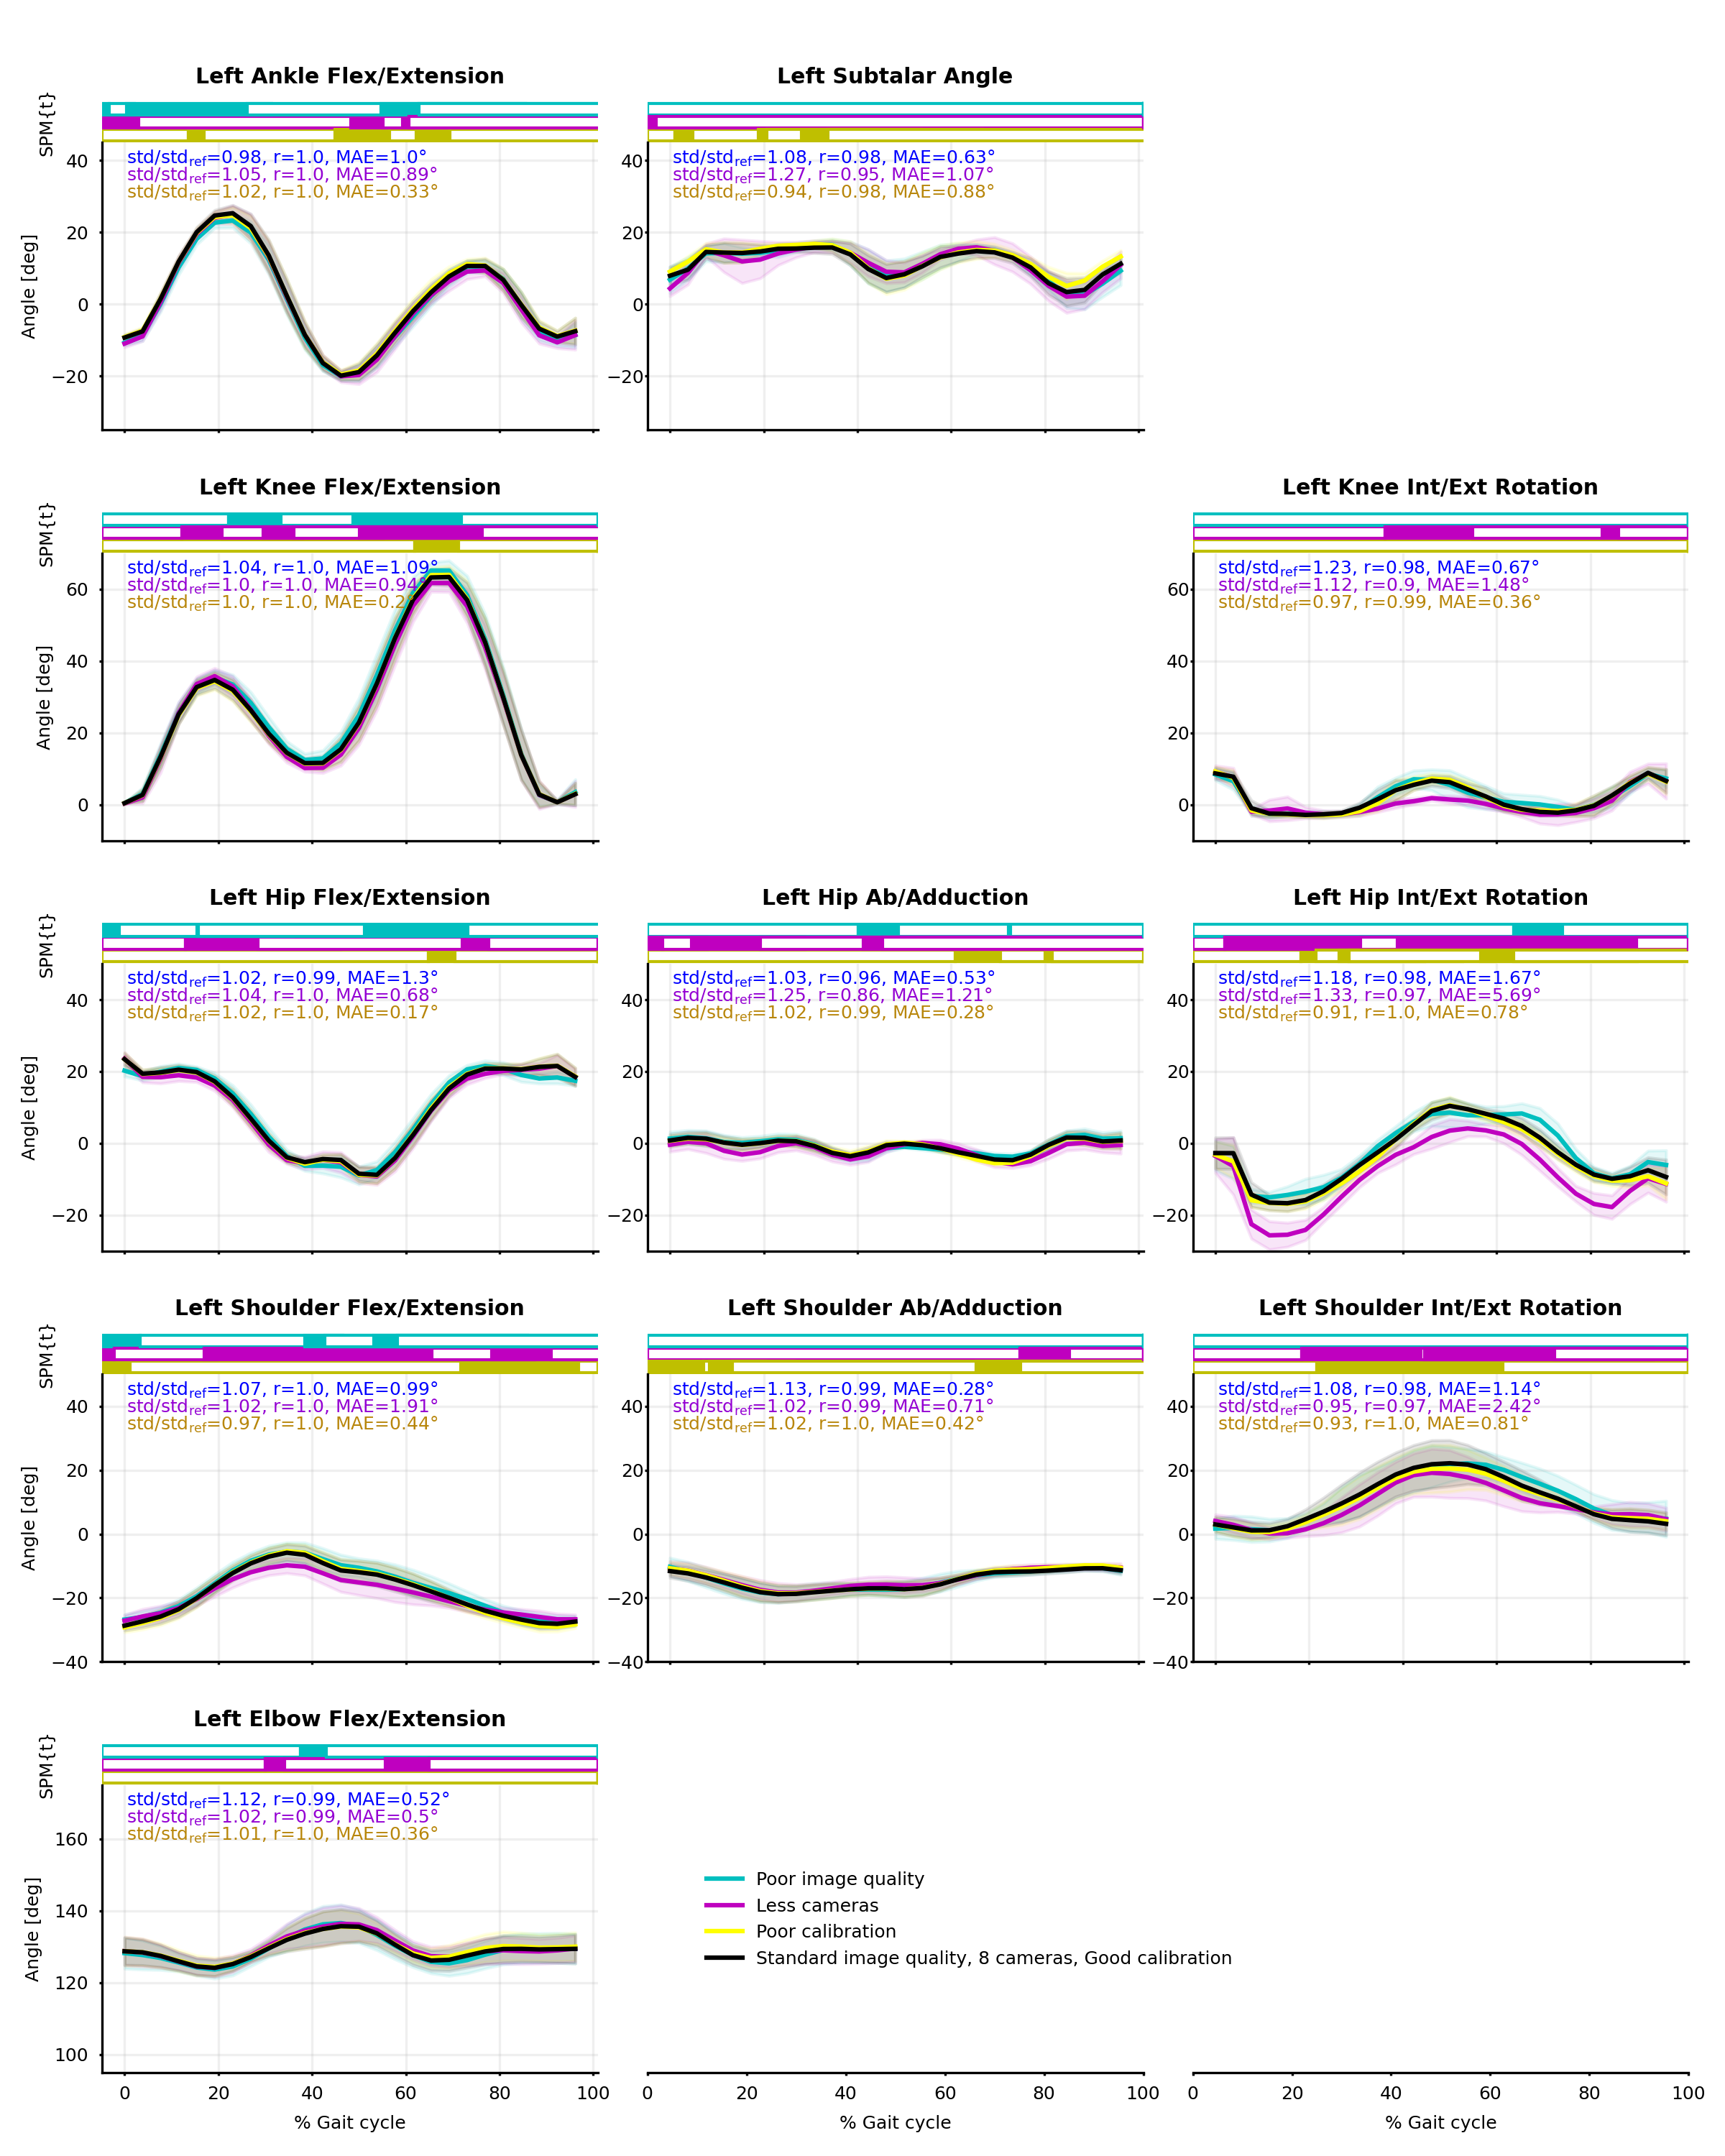
\includegraphics[height=\dimexpr\textheight-119pt]{"../Annexes/Figures/Fig_RunRobust.png"}
	\caption{Joint angle means (solid line) and standard deviations (shaded area) from the nine captured cycles of running. Reference condition (Ref) is black; degraded image quality (Im) is blue; four cameras instead of eight (4c) is purple; degraded calibration (Cal) is yellow. Pearson’s correlation coefficient (r) and mean absolute error (MAE) between Ref and Im, 4c, Cal were calculated. Paired t-tests along time were computed by SPM-1D and are represented as bar plots above the curves: a color rectangle means that there was a cluster of statistically significant differences (\(\alpha\) = 0.05) at that moment.}
	\label{fig_runrobust}
\end{figure}


\begin{figure}[!ht]
	\centering
	\def\svgwidth{1\columnwidth}
	\fontsize{10pt}{10pt}\selectfont
	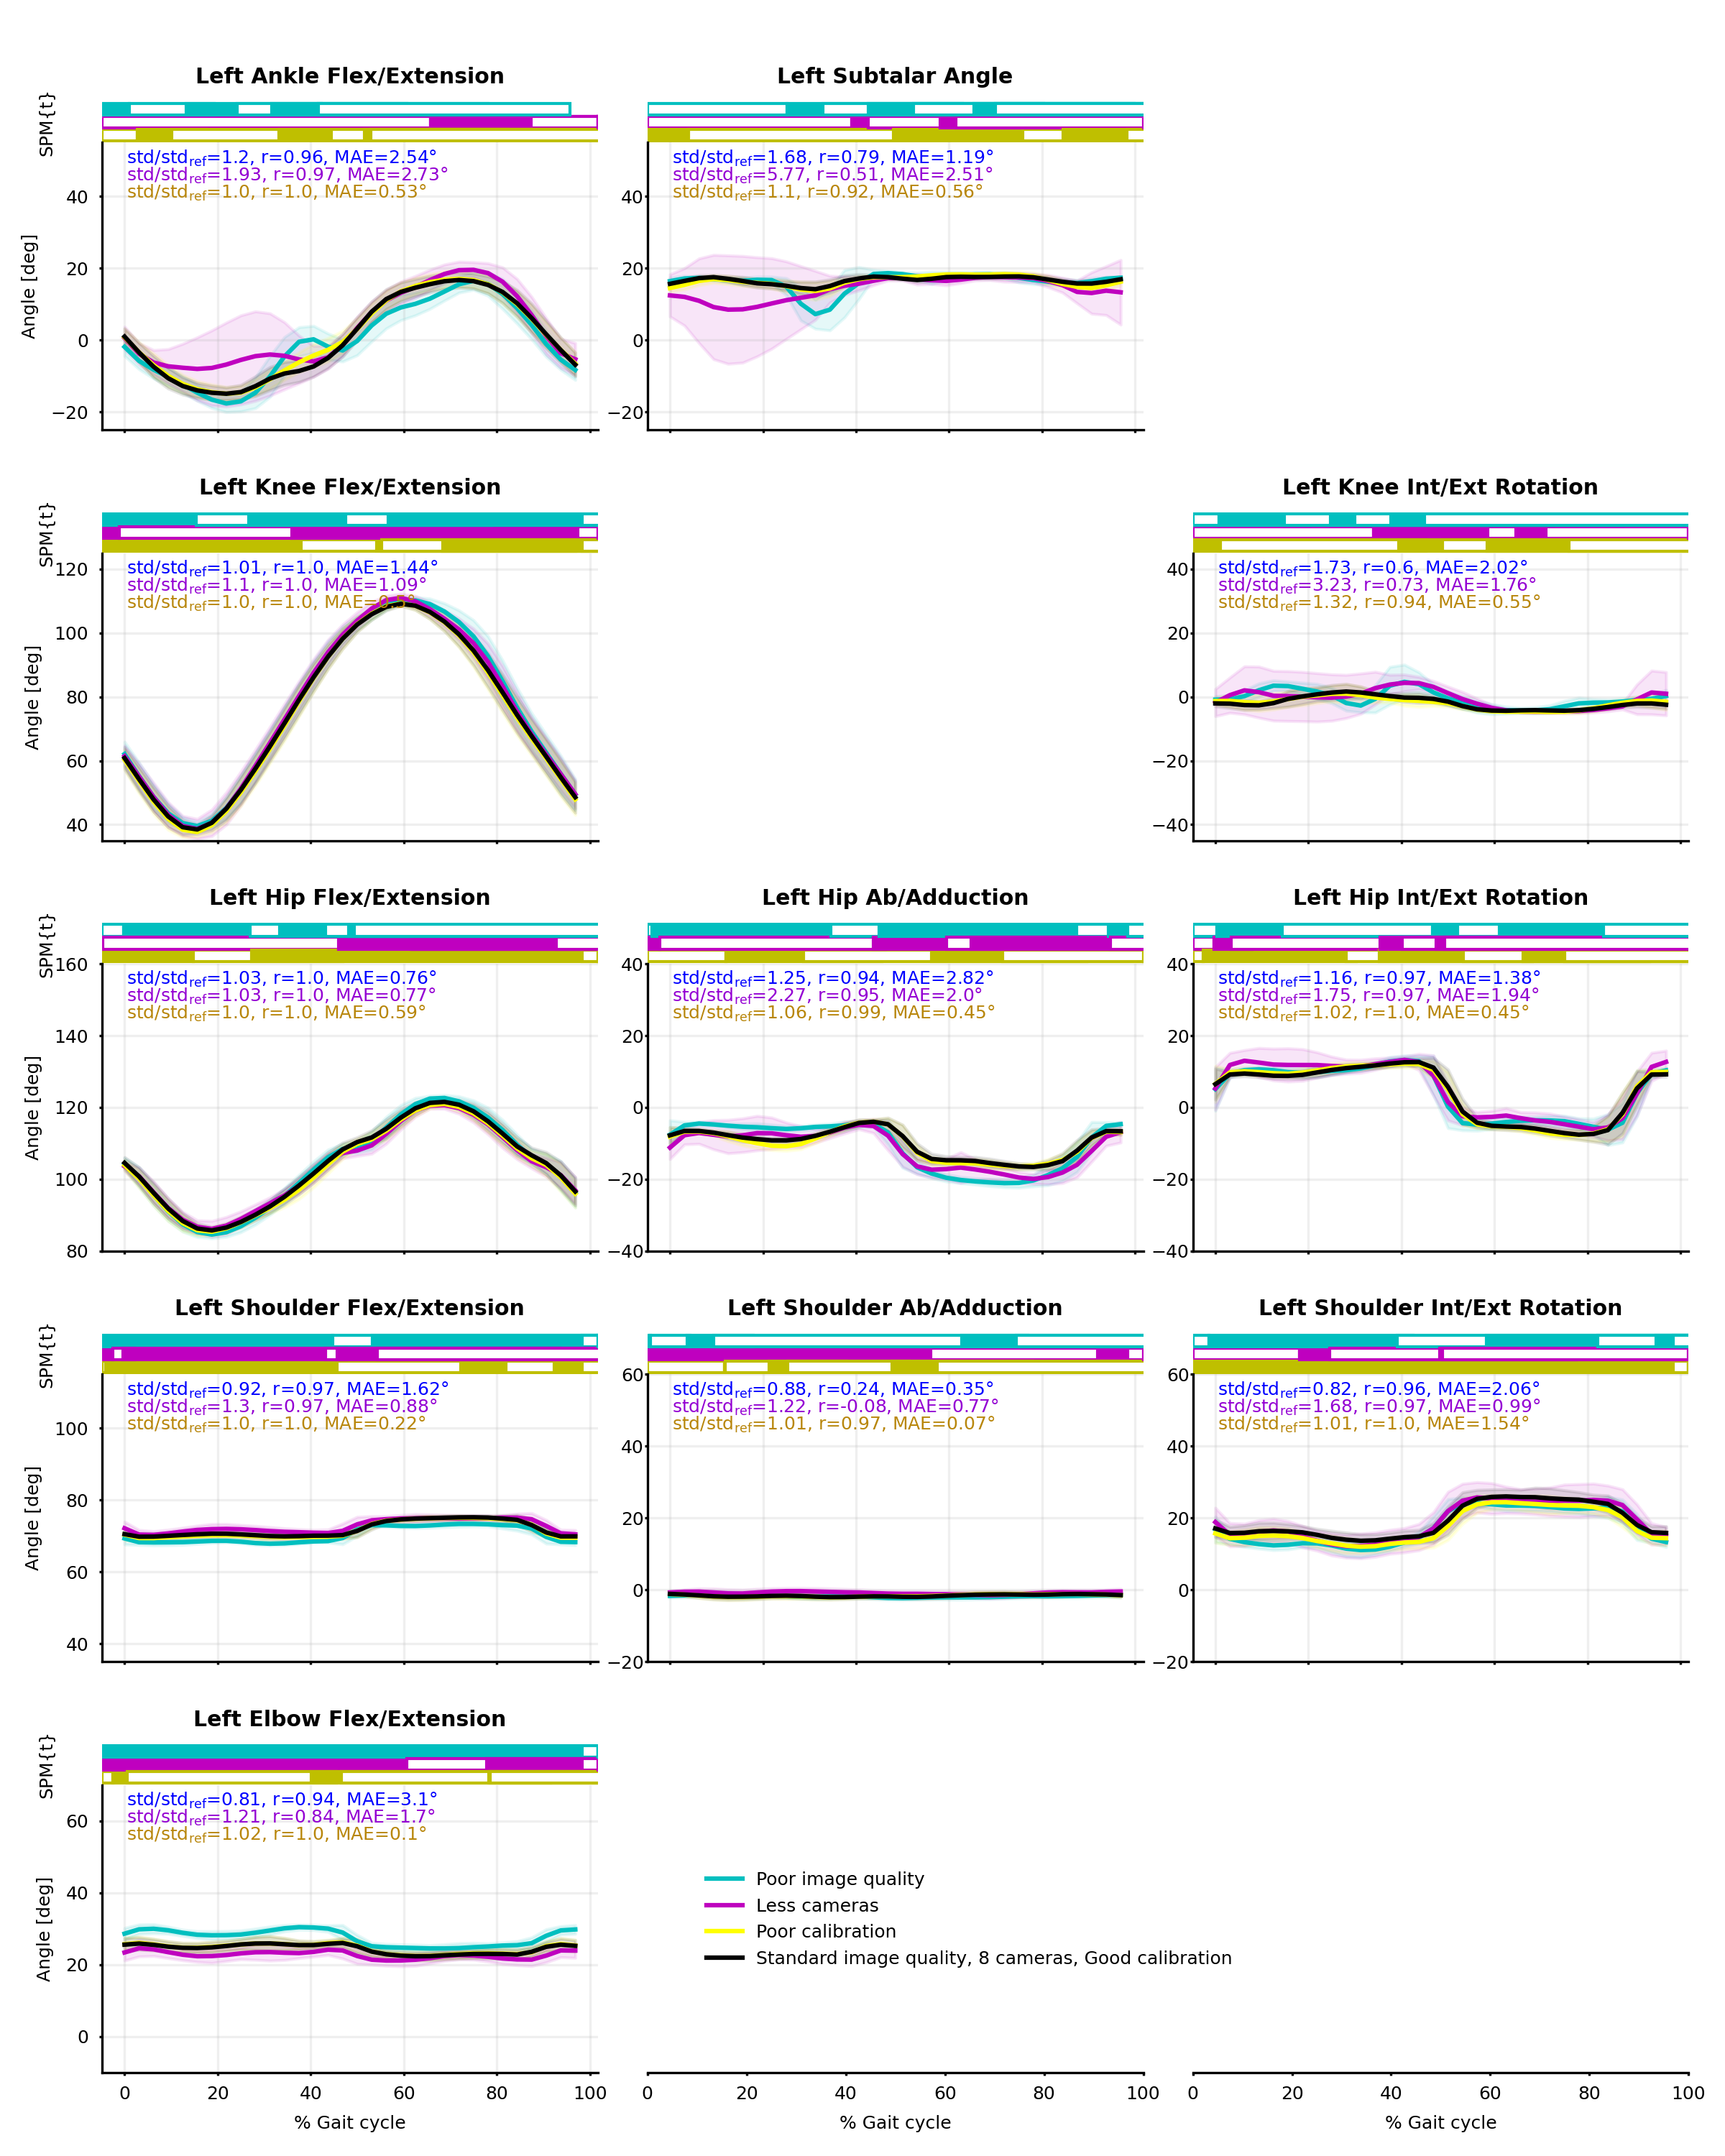
\includegraphics[height=\dimexpr\textheight-119pt]{"../Annexes/Figures/Fig_BikeRobust.png"}
	\caption{Joint angle means (solid line) and standard deviations (shaded area) from the 15 captured cycles of cycling. Reference condition (Ref) is black; degraded image quality (Im) is blue; four cameras instead of eight (4c) is purple; degraded calibration (Cal) is yellow. Pearson’s correlation coefficient (r) and mean absolute error (MAE) between Ref and Im, 4c, Cal were calculated. Paired t-tests along time were computed by SPM-1D and are represented as bar plots above the curves: a color rectangle means that there was a cluster of statistically significant differences (\(\alpha\) = 0.05) at that moment.}
	\label{fig_bikerobust}
\end{figure}


\FloatBarrier
\chapter{Appendix B : Title}
\label{Ann:2}

%==============================================================================	Résumé du chapitre

\begin{center}
\rule{0.7\linewidth}{.5pt}
\begin{minipage}{0.7\linewidth}
\smallskip

\textit{Summary here.
}

%\smallskip
\end{minipage}
\smallskip
\rule{0.7\linewidth}{.5pt}
\end{center}

\minitoc
\newpage


\section{Section 1}
\subsection{Sous section 1}
\blindtext
\subsection{Sous section 2}
\blindtext



\FloatBarrier
\chapter{Appendix C : Title}
\label{Ann:3}

%==============================================================================	Résumé du chapitre

\begin{center}
\rule{0.7\linewidth}{.5pt}
\begin{minipage}{0.7\linewidth}
\smallskip

\textit{Summary here.
}

%\smallskip
\end{minipage}
\smallskip
\rule{0.7\linewidth}{.5pt}
\end{center}

\minitoc
\newpage


Ajouter annexes :

Robustness

Accuracy

Protocole



\section{Section 1}
\subsection{Sous section 1}
\blindtext
\subsection{Sous section 2}
\blindtext



